\documentclass[a4paper,10pt,twocolumn]{article}
\usepackage[utf8]{inputenc}

\usepackage[T1]{fontenc}
\usepackage{gentium}

\usepackage{textcomp}
\usepackage{listings}
\usepackage{enumitem}
\usepackage{xcolor}
\usepackage{environ}
\usepackage{pdfpages}
\usepackage{amsmath}

\renewcommand{\abstractname}{\vspace{-\baselineskip}}

\newcommand{\PPODESUITE}{PPODE SUITE}
\newcommand{\MATLAB}{MATLAB}
\newcommand{\Fortran}{Fortran}

\newcommand{\shellcmd}[1]{\\\indent~\texttt{\footnotesize \$ #1}\\}
\newcommand{\matlabcmd}[1]{\\\indent\texttt{\footnotesize >> #1}\\}
\newcommand{\matlabcmdinline}[1]{\textacutedbl\texttt{\footnotesize#1}\textgravedbl}
\newcommand{\sourceword}[1]{\texttt{\footnotesize#1}}
\newcommand{\ph}[1]{\texttt{\footnotesize \textcolor{gray}{\textlangle #1\textrangle}}}
\newcommand{\filepath}[1]{{\footnotesize\textacutedbl #1\textacutedbl}}
\newcommand{\hyperlink}[1]{\emph{\footnotesize#1}}

\lstdefinestyle{fortrancode}{
  basicstyle=\fontsize{7pt}{1em}\ttfamily,
  frame=tb,
  backgroundcolor=\color[rgb]{0.99,0.99,0.99},
  escapechar=\%
}

\definecolor{darkgray}{rgb}{0.2,0.2,0.2}
\lstdefinestyle{matlabcode}{
  basicstyle=\fontsize{7pt}{1em}\ttfamily\color{darkgray},
  frame=tb,
  backgroundcolor=\color[rgb]{0.99,0.99,0.99},
  language=Matlab,
  commentstyle=\color{gray},
  keywordstyle=\bfseries\color{black},
  morekeywords={odeset, PPODE_build, PPODE_translate, ode15s, rigid, rigid_AM, @, e}
}

%opening
\title{\textbf{\PPODESUITE}\\Tutorial}
\author{Pascal A. Pieters\\\small{\textit{p.a.pieters@student.tue.nl}}}

\begin{document}

\maketitle

\begin{abstract}
\textbf{This document provides a small tutorial to get started with the \PPODESUITE. For more details on specific options or the internals of the suite, please read the \PPODESUITE~Manual provided with the package.}
\end{abstract}

\subsection*{Installation}
\paragraph{Dependencies}\mbox{}\\
The \PPODESUITE~currently only runs on Linux/Unix and requires \MATLAB~and GCC/GFortran to be installed. For details about the configuration of \MATLAB's MEX please consult the \MATLAB~help and forums. Note that using newer versions of GCC than officially supported by Mathworks generally does not cause any issues, so warnings similar to the following can be ignored.\\
\texttt{\small{"Warning: You are using gcc version \dots.  The version currently supported with MEX is \dots"}}\\
When MEX commands raise the error \texttt{\small{"\ph{\MATLAB~lib dir}/libgfortran.so.3: version 'GFORTRAN\_1.4' not found"}}, this can be solved by issuing the shell command: \shellcmd{sudo ln -sf \ph{GCC~lib dir}/libgfortran.so \\ \ph{\MATLAB~lib dir}/libgfortran.so.3} Where \ph{GCC lib dir} is for example \texttt{\small{"/usr/lib/gcc/x86\_64-linux-gnu/4.8"}}.

\paragraph{HPC ICMS Cluster}\mbox{}\\
On the \textit{HPC ICMS} cluster, all dependencies are already installed. \MATLAB~is however not correctly configured to use GFortran. This can be solved by issuing: \shellcmd{echo -e "{\textbackslash}nalias g95=\textbackslash"gfortran\textbackslash"{\textbackslash}n" {>}{>}\\ $\sim$/.profile \&\& source $\sim$/.profile}

\paragraph{General}\mbox{}\\
Unpack the \PPODESUITE~package, the created directory will be referred to as \ph{Install Path} from hereon.
\shellcmd{tar -xzf PPODESUITE-0.*.tar.gz}
Open \MATLAB~and change directory to the \ph{Install Path}.
\matlabcmd{cd \ph{Install Path}}
Build the libraries of the \PPODESUITE~package.
\matlabcmd{PPODE\_init}
This concludes the installation, for next sessions it will suffice to change directory to the \ph{Install Path} and run the addPaths script to add the \PPODESUITE~paths to the \MATLAB~path variable.
\matlabcmd{PPODE\_addPaths}

\paragraph{Startup}\mbox{}\\
To automatically load the \PPODESUITE~paths into \MATLAB~upon statup, start \MATLAB~as root:
\shellcmd{sudo matlab}
And edit the startup script using the command:
\matlabcmd{edit startup}
Add the following lines to the file:\\\\
\texttt{\small{addpath '\ph{Install Path}'\\
PPODE\_addPaths}}

\subsection*{Prepartion}
In \MATLAB, change directory to the path of the \MATLAB~ODE file that should be evaluated using the \PPODESUITE. Open the file that contains the ODE definitions, i.e. the function file that is usually supplied as first argument to the \MATLAB~ODE solver (\matlabcmdinline{ode15s(@\ph{odefunc}, ...)}, which is defined in the file \ph{odefunc}.m). This function definition should have a header of the following form:
\matlabcmd{\ph{dx} = func( \ph{t}, \ph{x}, \ph{par}, \ph{neq}, \ph{np} )}
Where \ph{t} is the independent variable, \ph{x} the dependent variable(s) and \ph{par} the parameter values. The last two arguments are optional and represent the number of equations (\ph{neq}) and number of parameters (\ph{np}). For further restrictions on the ODE function, see the \PPODESUITE~Manual.

If the function fullfills the requirements of the \PPODESUITE, it can be parsed to the programming language of the \PPODESUITE~(\Fortran~95).
\matlabcmd{PPODE\_translate('\ph{odefunc}')}
This function will generate the file '\ph{odefunc}.F', which can be build against the solver libraries provided.
\matlabcmd{PPODE\_build('\ph{odefunc}.F', '\ph{execID}')}
Where \ph{execID} can be any identifier for the executable, e.g. 'odefunc\_StiffSolver'. This command does not specify any options, so all default values will be used. Therefore also the default solver is used, which is a fully automatic solver, for the use of other solvers consult the \PPODESUITE~Manual.

\subsection*{Execution}
The ODEs can now be solved by calling the executable generated by the build command.
\matlabcmd{[\ph{t}, \ph{y}] = \ph{execID}(\ph{neq}, \ph{abstol}, ...\\ \ph{reltol}, \ph{times}, \ph{par}, \ph{y0})}
Where \ph{neq} is the number of equations, \ph{abstol} and ph{reltol} are the absolute and relative tolerances respectively, \ph{times} is a vector of time points at which output is desired, \ph{par} is a vector of parameter values and \ph{y0} is a vector of the initial values of the states. The function returns the vector \ph{t} with the time points at which the values of the states are calculated. The matrix \ph{y} contains the values of all states at the time points specified by \ph{t}.

Note that the number of equations (\ph{neq}) has a special role in the \PPODESUITE, since it was developed to work with large systems of ODEs that can have a variable number of equations. Therefore, it is important to always provide a correct number of equations. So if a system has a fixed number of equations, this number still has to be supplied. An easy way to do this is to use the size of the intial values, i.e. provide \matlabcmdinline{length(\ph{y0})} as first argument.
% 
% \section{Sparse Jacobian}
% One main feature of this suite is the ability to solve large systems of sparsely interlinked ODEs. These systems can be solved - within reasonable amount of time - by solvers that make use of a sparse Jacobian matrix implementation. These solvers require the user to provide a number of nonzero elements of the Jacobian matrix. To let \PPODESUITE~calculate this number, a Jacobian function has to be generated from the \ph{odefunc}. This can be done by providing the 'AnaJac' option to the translate function.
% \matlabcmd{PPODE\_translate('\ph{odefunc}', 'AnaJac', 1)}
% Subsequently, the ODE system has to be build against the correct solvers. The \PPODESUITE~provides two solvers that make use of a sparse Jacobian matrix, namely 'LSODES' and 'MEBDFSO'. To build the system against for example the 'LSODES' solver, the following build command can be used:
% \matlabcmd{PPODE\_build('\ph{odefunc}.F', '\ph{execID}', ... \\ 'Solver', 'LSODES')}
% All other steps stay the same with respect to what was described before.

\subsection*{Example}
An example of this workflow can be found in the \filepath{examples/rigid} folder of the package. The function \matlabcmdinline{compareSolvers} evaluates a simple stiff problem using various solvers. The ODEs are defined in the file \filepath{rigid.m}. The \matlabcmdinline{compareSolvers} function nicely shows the differences between the use of a \MATLAB~ODE solver and the \PPODESUITE.
\vspace{1cm}
  \begin{lstlisting}[style=matlabcode,caption=Code Snippet]
PPODE_translate('rigid');
y0 = [0 1 1];
par = [-0.51];
t = 0:0.01:20;
options = odeset('RelTol', 1e-4, 'AbsTol', 1e-4);

% The ode15s solver
[t1, y1] = ode15s(@(t,y)(rigid(t, y, par)), ...
                   t, y0, options);
% The Adams-Moulton solver
PPODE_build('rigid.F', 'rigid_AM', ...
             'Solver','Adams-Moulton');
[t2, y2] = rigid_AM(length(y0), ...
                     options.AbsTol, ... 
                     options.RelTol, ...
                     t, par, y0);
                     
figure(1);
subplot(2, 1, 1);
plot(t1, y1(:, 1), 'r-', t1, y1(:, 2), 'g-', ...
      t1, y1(:, 3), 'b-');
xlabel('t');
ylabel('y(t)');
title('Rigid Example - ode15s');
subplot(2, 1, 2);
plot(t2, y2(:, 1), 'r-', t2, y2(:, 2), 'g-', ...
      t2, y2(:, 3), 'b-');
xlabel('t');
ylabel('y(t)');
title('Rigid Example - AM');
\end{lstlisting}
The output of this code is:
\begin{figure}[hb!]
 \centering
 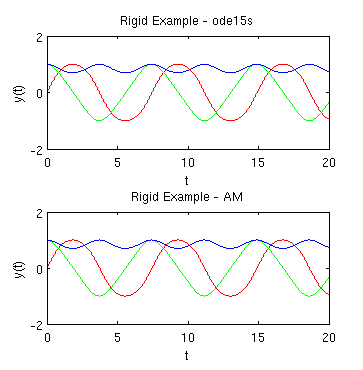
\includegraphics[width=0.35\textwidth]{./RigidSolution.png}
 % RigidSolution.png: 368x431 pixel, 90dpi, 10.39x12.16 cm, bb=0 0 294 345
\end{figure}

\end{document}
